%!TEX TS-program = xelatex
    %!TEX encoding = UTF-8 Unicode
%    \documentclass[10pt, letterpaper]{article}
\documentclass[letterpaper,10pt,oneside,headsepline]{scrreprt}
\usepackage{fontspec} 
\usepackage{placeins}
\usepackage{multibbl}
\usepackage{graphicx}
\usepackage{txfonts}
\usepackage{url}
\usepackage{xltxtra}
\usepackage{geometry} 
\usepackage{pdfpages}
\usepackage{amssymb}
\usepackage{makeidx}
\usepackage{paralist}
\usepackage{comment}
    \geometry{letterpaper, textwidth=5.5in, textheight=8.5in, marginparsep=7pt, marginparwidth=.6in}
    %\setlength\parindent{0in}
    \defaultfontfeatures{Mapping=tex-text}
    \setromanfont [Ligatures={Common}, SmallCapsFont={ITC Officina Serif Std}, BoldFont={ITC Officina Serif Std Bold}, ItalicFont={ITC Officina Serif Std Book Italic}]{ITC Officina Serif Std Book}
    \setmonofont[Scale=0.8]{Lucida Sans Typewriter Std} 
    \setsansfont [Ligatures={Common}, SmallCapsFont={ITC Officina Sans Std}, BoldFont={ITC Officina Sans Std Bold}, ItalicFont={ITC Officina Sans Std Book Italic}]{ITC Officina Sans Std} 
\usepackage[ngerman,english]{babel}
\usepackage{scrpage2}
\clubpenalty=6000
\widowpenalty=6000
\author{Avery Laird}
\title{Southridge Tech Manual}
\date{\today}
\ohead{Southridge}
\chead{Tech Manual}
\pagestyle{scrheadings}
\setcounter{secnumdepth}{-1}
\makeindex
\begin{document}

\pagestyle{empty}
\vspace*{7em} 
\begin{center}
\huge{Tech Manual}\\
\vspace*{1em} 
\large{Southridge School}
\end{center}
\clearpage
\pagestyle{scrheadings}
\tableofcontents
\newpage
\section{Acknowledgements}
Amaan Mawji, \\ Traven Blaney, \\ Spencer Reichert. \\ I couldn't have written all this without your help. \\ This manual was written entirely in \XeLaTeX. \\ 
\section{How to read this book}
If you're reading this sentence then you've pretty much got it. \\ Good job. Just keep going the way you are.

\chapter*{Preface}
\begin{flushleft}
\begin{quotation}
Fail to honour people,
They fail to honour you;
But of a good leader,
Who speaks little,
When his work is done,
His aims fulfilled,
They will say,
"We did this ourselves."

- Lao Tzu
\end{quotation}

\end{flushleft}

I believe this quote beautifully describes the fine balance one must juggle when given the responsibility of Tech Steward. What did Lao Tzu mean by "fail to honour people"? Is it because you didn't shower them with praise, or shove them in the spotlight for a task they accomplished? I don't think so. To me, he meant that if you don't respect people, you will never gain respect in return. This is very, very important: as a Tech Steward, you must be respected by your peers and colleagues on the team, and hopefully out of the team. Of all the duties you must accomplish, this will be the hardest, because respect is something that must be earned; it can't be bought or taken. You have to honour people, and in return, they will honour you. Next, what does this weird sentence mean here, "But of a good leader / Who speaks little"? It means a lot of things. First, he says that a good leader is not one who speaks a lot about all these wonderful things we should do -- then when it comes to accomplishing those things, it all goes up in smoke. A good leader guides, and, well, leads! He or she gives everyone on the team the tools to accomplish what needs to be done, but does not do everything for them. Then, "When his work is done / His aims fulfilled / They will say / "We did this ourselves". Of course, the irony of this situation does not elude me -- here I am, a leader, telling you that a good leader doesn't tell people what they should think! That is why I want you to study the above quote, and study it hard, then draw your own conclusions. What I have written here is a guide, a tool - and it's completely imperfect. There are any number of things that can be changed to be more efficient, and it's your job to decide what you want to make better, because that's what our role really is here - to make the position of Tech Steward better than how we left it.

\chapter{General}
\textit{Safety}: In the tech team, Safety is our number one priority. You've probably heard a lot of stories, and I'm probably in some of them. However, something you probably don't know is that the whole time, we were being completely safe. There are a lot of things we do on the tech team that are dangerous, and that's because they can be, if you don't use the proper safety techniques. A lot of the things we do sound unsafe, like hanging the Country Fair speakers with gaffer tape, and that's why they make very entertaining stories -- but they are totally safe as long as you don't do anything to compromise that safety. That could be something you do unknowingly, which will happen accidentally but should be avoided at all costs. Mistakes will happen, but that doesn't stop you from doing all you can to prevent them, especially when it comes to safety. Safety could also be something you compromise knowingly. I cannot stress this enough: never cut corners. EVER. I don't care if you are under pressure to get something done, whether it be on time, on budget or with the least amount of work. You must NEVER give in to that pressure. Sometimes that means telling someone that you can't get it setup that fast, or that it's going to cost them a bit of extra money -- and although that's never terrific, it will always be better than someone getting hurt.

\subsection{Safety Equipment}
\index{Harness}A harness should always be used when you're doing something high up and exposed. It shouldn't be used on a scissor or \index{bucket lift}bucket lift, but for \index{rigging}rigging and hanging purposes. It is almost always best to use the \index{five-point harness}5-point harness rather than the lower body harness. You can only stay in a lower body leg-loop harness for about 20 minutes before circulation is completely cut off to the lower body. For a 5 point harness, that time is greatly extended. For harness information, see page. As for other safety apparatus, none are used daily or even yearly. For any more information you would need regarding safe usage, consult the section of the individual event.
\begin{comment}
A page reference is missing above.
\end{comment}


\subsection{Attitude}
The tech team has a reputation of being hardworking and somewhat eccentric. In my opinion, this is totally okay -- as long as it doesn't go too far. For example, there's a story in which some previous members bought a fibre optic lamp, the ones with the lit strands. When someone came over and fiddled with it, they started exclaiming not to touch it, because it was some kind of "sophisticated communication device." Hilarious? Of course! Respectful? It depends. These types of pranks are funny once in a while, and I'm by no means saying you should never have the odd joke. Hopefully, the tech team has many in-jokes; that's what makes it enjoyable and fun. However, it's all about intention. You've got to ask yourself whether the joke has a malicious intent, or is just a good natured piece of humour (the latter is very important in the tech team).

Another attitude point I'd like to stress: \textit{do not point fingers}. On the tech team, \textit{things will go wrong.} Sometimes it's not our fault, sometimes it is, but it doesn't matter. Placing the blame is not going to fix anything, or get the slideshow going any faster. People also make mistakes -- and they probably are already all too clear they screwed up. So, as a closing note, be tolerant, patient and keep a cool head. If you freak out, it can make a domino effect, and things will start to fall apart at the seams. If the leader has a cool head, then the team calms down and will prevent anything else from going wrong.
\chapter{Events}
Now we're into the heavy stuff: a list of all the major events throughout the year, equipment required, techniques and tips. Let's begin.
\section{Assemblies}
I put the assemblies first because this is the event you do the most throughout the year, twice a week. Although you'll do this event the most by far, it's in some ways the most challenging. Since the assemblies are never planned all the way through in advance, that means there's almost always something unexpected. This is why you should \textit{always have someone experienced at the hog.} They need to be someone who can improvise, troubleshoot on the fly and basically make it work when something goes wrong. Also have someone learning the hog sitting with them, to lend a hand and learn problem solving techniques when under pressure. It's the perfect venue to learn because there's a certain amount of pressure present, but it's also more casual, so if something absolutely does not work, it's not as important as when bad things happen at a more upscale event, such as the play. The same goes for the sound cabinet. 

\section{Assembly Configuration}
Assemblies usually consist of these elements:
\begin{enumerate}
\item On the first assembly of the week, we sing O Canada.
\item Address from head of school.
\item Teacher announcements.
\item Student announcements. 
\item Dismissal.
\end{enumerate} 
Typically, it's just a stage wash for the majority of the assembly, except for student announcements (they're held on the left-hand side of the Great Hall).

\section{Full School Assembly}
Besides the normal assemblies, this is the event you'll find yourself doing the most. The basic setup procedure goes as follows:
\subsection{Gymnasium Lamps}
\begin{enumerate}
\item Find NSI Lighting Console. On how to program the board, see "NSI Lighting Board Operation."
\item Plug one XLR into the control panel located near the window for the P.E. offices, which are by the gym P.A. cabinet.
\item The MALE end goes into the control panel, and the FEMALE end connects to the console. That is \textit{very important}.
\item Up all of the channels, and take note of which lights respond. I like to number the lights from left to right in my head.
\item Grab someone to stay in the gym with a radio, and then head up to the tech room.
\item Once in the tech room, start with the "A" patch. Say, "Plugged in!" over the radio. The person in the gym should say, "That's it!" or, "On!" if the patch powers up one of the lights. If not, they should say, "Nope!" or, "Negative!" -- something along those lines. (This is the procedure I will use until I have mapped out all of the active circuits, which will hopefully be soon.)
\item Once you have cycled through all of the patches, all of the lights should be on. Good job! If not, something is wrong. Time for some good ol'fashioned troubleshooting. For general troubleshooting tips, see "Troubleshooting." I'll explain the specific troubleshooting next.
\end{enumerate}
\subsection{Gym Light Troubleshooting}
For a beginner, the lights in the gymnasium are quite possibly the most complicated, temperamental and screwy pieces of equipment you'll ever have to deal with. They're an enormous pain! However, there is a way to tame the beast. Once you've figured out the naunces of the setup, you and the lights can hug, kiss, makeup and be friends forever. The more you know about how the setup works, the better you can troubleshoot. Do this troubleshooting enough times, and you can guess the problem almost right away. Let's start with how everything fits together, in order from lighting console to dimmerpack:
\subsubsection{Microplex (Data)}
\begin{enumerate}
\item XLR from console to utility panel.
\item XLR from the outlet of the utility panel, up and along the ceiling of the gym to the far back right side and to the ceiling of the tech room.
\item XLR from the ceiling of the tech room to the dimmerpack.
\end{enumerate}

\subsubsection{Circuit (Power)}
\begin{enumerate}
\item Dimmerpack to the ceiling of the tech room.
\item Through the ceiling of the tech room to the ceiling / girders of the gym.
\item From the girders to the various outlets on the girders.
\item Outlets to lamp.
\end{enumerate}

Now that you know this information, see what you can do to find the source of the problem. Some common problems to check for are blown bulbs and ripped plugs. That about does it for lighting. On to sound.

\subsection{Gymnasium Sound}
This is a bit of a tricky one too. The first thing you need to do is figure out how many mics are needed, because most of the time you can get away with just using the wireless mics. Next, make sure you talk to Mr. Burrage a few days in advance. I can count a few times when, 20 minutes before the full school, someone will suddenly remember the whole choir's singing. It can be very humorous, but not very useful information when you're scrambling for eight mics and trying to haul that huge onyx mixer through the hall, plus the snake, the other XLR -- you get the idea. So, bottom, line, the first thing you've got to do is figure out how many mics you need. If you need more than 2 wireless mics, you can grab some more from the P.A. cabinet in the great hall. Overall, if you need more than 4 you've got to bring out the big guns. For the choir, \textit{always use a separate mixing board}.

Let's say the choir's playing. The first thing you need to do is, once again, figure out how many mics they need. Normally it's eight. Then, grab x amount of mics, the same amount of XLR, the snake, a mixing board and bring it back to the gym. Set it up on one of the cafeteria tables. Plug the snake into the patch panel by the gym P.A. cabinet, 1--8 (I usually do 4--12, don't ask me why). Then, into the mixer. Next, go to the stage and layout the mics. Plug the XLR in the mics, then into the corresponding patches by the stage. Plug the mixer into the cabinet on an unused input (usually iPod is the best). Next, route \textit{everything} through the mixing board (except for the onboard mics). Ever watch Star Trek? \textit{Route all power to shields!} No? Anyways, now everything but the two onboard mics should be routed and controlled through the separate mixer. Start a mic check on all mics, then move on to the next step.

Now we can start on the piano and computer cart. For the piano, find any which way to convert the quarter-inch output to XLR input. Usually you use a quarter-inch to female, then a female to female coupler, then patch it though the front panel, through the snake and into the mixer. The same for the computer cart, although usually it has a straight male XLR output. Now, if you're going to get hum, it's going to be about 99 per cent likely that it's the computer cart or the piano. (That's definitely a proven scientific statistic..). Just to be sure, I always put a hum eliminator on the computer car and the piano.

I think that does it for sound. Next, Video.

\subsection{Gymnasium Video}
You're in the home stretch. This is the relatively easy part, because the projector just has a nice, simple VGA input. There you have it, the full school assembly.

\subsection{Wrapping up}
That should just about do it for the full school assembly. This is a difficult event, and there's always something unexpected no matter how many times you do it. Just remember that mistakes happen. Just figure out how they happen and learn from them so that you can prevent them in the future.

\section{Mid-September: Terry Fox Run / House Picnic}
The house picnic is usually more low key and fun, but we still need to deliver clear and audible music and P.A. announcements. That's actually really hard to do; the StagePass 500's just don't cut it for outside; they're an inside P.A system. Once you get out about 15 metres, the sound just cuts off and is really hard to hear. Unfortunately, until we get more powered speakers the SP500's will have to do. Here's how to squeeze out the most bang for your buck:
\subsection{Speaker Positioning}
\begin{enumerate}
\item \textit{Avoid involuntary noise cancellation.} If you remember your physics classes, you'll know that light waves with the same peaks and valleys cancel each other out, which is why the light-slit experiment is so famous (they deduced light was both a particle \textit{and} and a wave.) The same goes for sound. The pressure waves coming from the speakers are almost exactly the same when they leave the speaker. In the wrong position, you might accidentally cancel out the waves, limiting how much sound the speakers produce. You can avoid this by making sure the speakers don't cover the same area; it's overkill, \textit{and} it can cancel out the sound.

\begin{comment}
Isn't is opposite waves that cancel each other out?
\end{comment}

\item  \textit{Power Source.} The power at the park is coming from one outlet only, so you can't spread the speakers out much. Try and think about the most useful layout; for example, avoid an overlap in sound direction as much as possible.
\end{enumerate}

Next, we'll talk about how to configure the onboard mixer to get the most out of the SP500's.
\subsection{SP500 Mixer Configuration}
The mixer on the back of the SP500 is quite simple. Here's a picture: 
\begin{figure}[ht]
\centering
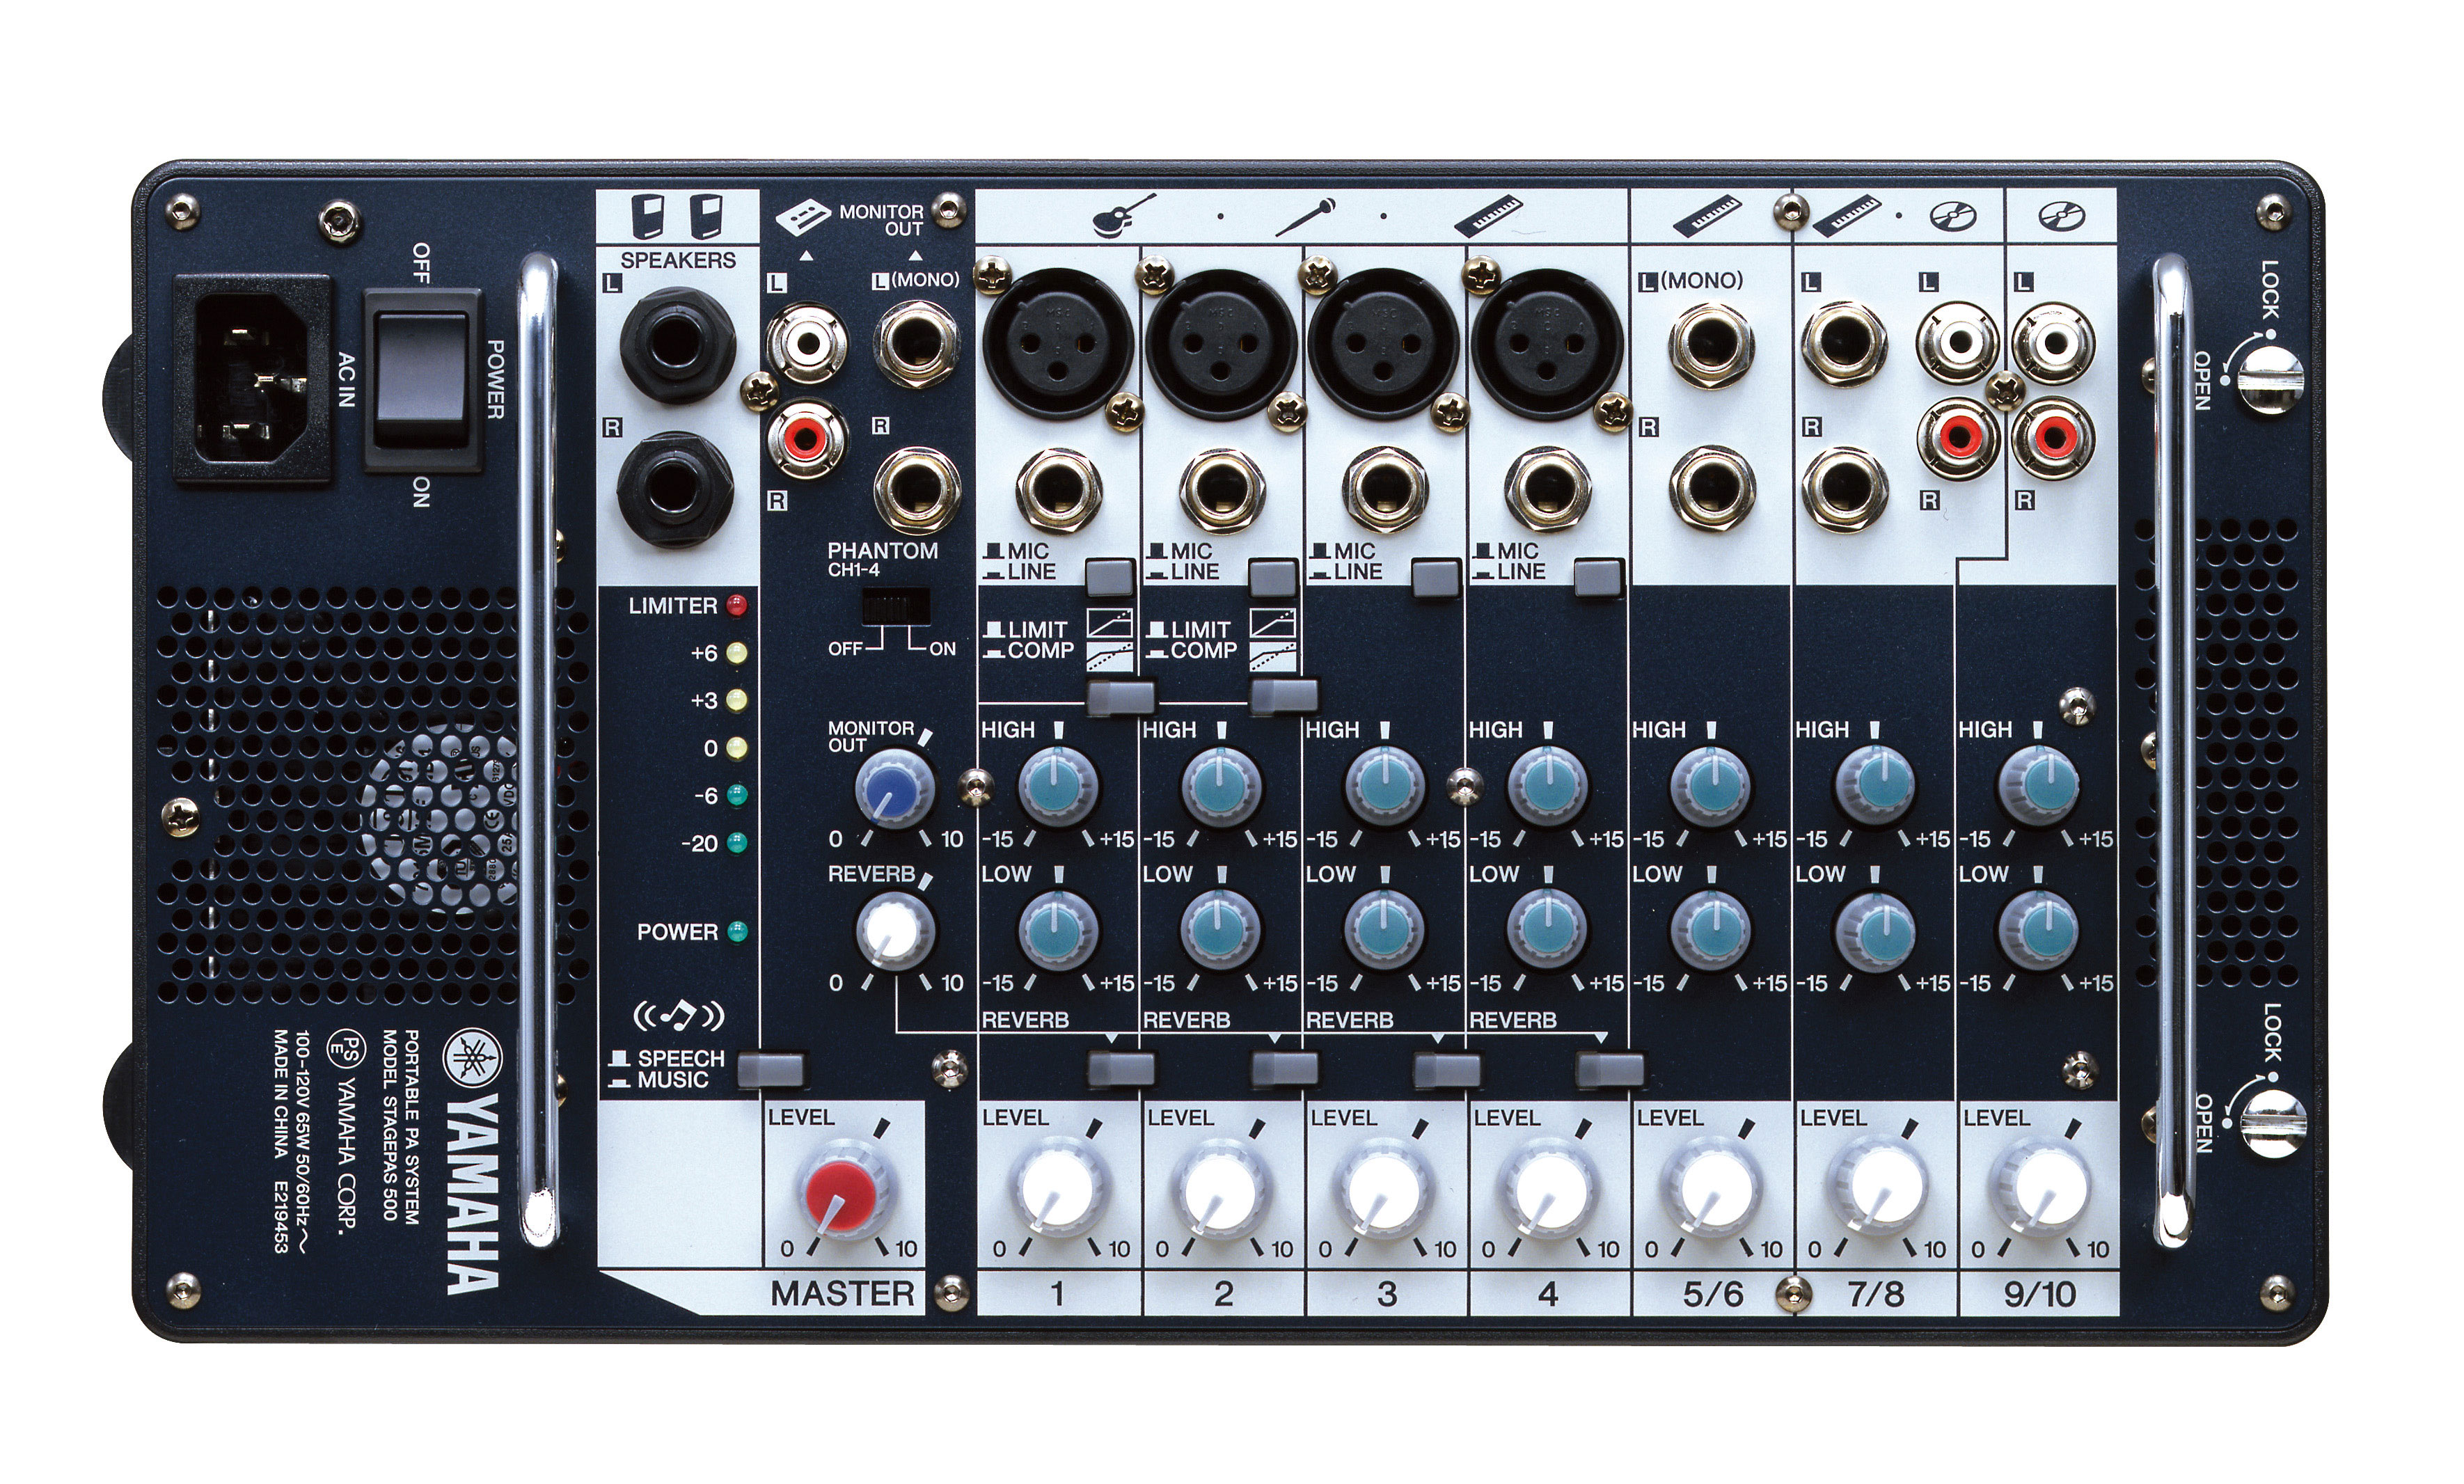
\includegraphics[scale=1]{STAGEPAS500_07} 
\end{figure}

Now depending on the climate of the day, you won't mind pushing it to the limiter. The speakers may heat up a bit, but the limiter is exactly that: it limits the output so as not to damage the speakers. However, you will soon find that upping the gain will appear to boost the output. \textit{This is not advised!} It \textit{will} damage the speakers. Keep the gain low to avoid distortion, and if the limiter's lighting up for most of the time, it's too loud. That's really the most you can do, and once you've reached that level of peak output, stop tweaking, because it won't get any louder, trust me. As for music, I usually just bring a radio along and set it to a popular station. There you have it, the Terry Fox Run and House Picnic.

\section{End of October: Manning Park Jazz Retreat}
Manning Park is always a fun venue to work, and the setup and operation are simple too. Depending on the year, you'll require different equipment, but the following is a list of what I usually use. \textit{Be advised:} The following numbers change from year to year, and do not account for spares. Always be sure to bring at least one or two spares of smaller equipment (microphones, cables, couplers, etc).
\subsection{Equipment List: Manning Park Jazz Retreat}
\begin{enumerate}
\item \textit{2} JBL passive speakers
\item \textit{2} Cases for JBL powered speakers
\item \textit{Minimum eight} Shure Beta 58A Microphones (check how many are needed with Mr. Burrage)
\item Black gator case
\item Microphone stands (number can differ greatly, but usually around \textit{5 -7} with a majority of booms)
\item \textit{2} Speak-on cables
\item Mixer and amplifiers. This is also up to you, because it depends on whether you want incredible sound quality or ease of use. In this case, since the new mixer is quite large and tricky to move in the van, I recommend the mixer rack in the band room.
\item XLR cables. This depends on how many microphones you bring, but it's a good idea to bring at least \textit{10} XLR.
\item \textit{2} hum eliminators.
\item \textit{1} JDI box.
\end{enumerate}
This is the bare minimum for tech. Usually Mr. Burrage also brings power, patch cords, etc. However, \textit{every year you have to confirm this, in advance.} If you don't, he might not bring them and then you're in a sticky situation. A few weeks in advance, you must discuss all of this with Mr. Burrage. That way, you can coordinate supplies and avoid overlaps and oversights.
\subsection{Setup} 
Setup is something that you're going to want to do as soon as possible when you arrive at Manning. Often what we'll do is arrive the day before and setup the system. For example, we might leave around 4:30 / 5, arrive around 10 and I'll setup until 11 or 11:30. That's more than enough time to finish all that's needed. My rough method for setting up is as follows:
\begin{enumerate}
\item Remove JBL's from cases, and turn cases on their sides. Then stack JBL's on the cases. The best position for the speakers is two behind the playing area, facing in towards the audience. Be sure not to blast these speakers, as you may experience feedback.
\item Unpack the mixer and position it at the back of the room. Plug it in and test to make sure it turns on properly, then turn it off.
\item Run the speak-on cable from the far right speaker to the left speaker.
\item Run the speak-on cable from the left speaker to the "Bridge" output of the amp.
\item Run an XLR cable from the mixer to a microphone for use as a talk-back and testing input. You can also use something like an MP3 input, but I recommend a microphone.
\item Test the speakers using the microphone, and troubleshoot to solve any problems.
\item Wire the rest of the microphones to the front of the stage area, and mount some of them on the stands.
\item Test all of the microphones, and set levels.
\end{enumerate}

\subsection{Wrapping up}
As with all off-location venues, there is a lot of compromising and problem solving involved with Manning Park. However, as long as you do your best to plan ahead, check and triple check and bring backups, you should be fine. Things beyond your control may happen, but at least you know you tried your best to prevent any miscommunications or accidents. Other than that, remember to enjoy it.

\section{Mid-November: Gala}
To be fully honest, there's not much to say about the Gala. It truly is on a case by case basis, and since we only have it at Southridge every other year, it's not even an annual event. There is not a large tech focus. The most you'll likely have to do is re-aim the gym lights to add illumination and program a funky light show in the Great Hall.
\section{Mid-December: Winter Concert}
The Winter Concert is big (we only have two concerts per year). Accordingly, this section is split up into lighting, sound and video sections. For the rental equipment setup, see the followig sections on Shears, LED Blasters, and the Hazer. 
\subsection{Lighting Overview}
Lighting is a very important aspect of the winter concert. Much effort is put into improving and expanding on the equipment we have, and renting new equipment. Attached on the next page is an invoice for equipment we almost always rent every year, consisting of shears, LED blasters and a hazer. We can review the techniques to fully utilize the blasters in a bit. Another very important aspect of the lighting for both the concerts is making the VL1000's look as beautiful as possible (another thing we'll discuss in more detail later). All of the following steps such as the renting of equipment and design of the show should be organized as soon as possible, ideally about a month before the show. You can always order the equipment for a certain date far in advance, and this ensures that you receive the equipment at the same price with the same quality.

\subsection{sample rental invoice}
%\includepdf[pages=1]{/home/avery/Downloads/Winter_Concert_invoice}
\begin{comment}
I have commented out the graphic above because it's not in the repo.
\end{comment}

You can see from the above the equipment usually rented for the Winter concert. In the next section I'll go over how to set it up, and then offer some tips for designing the show on the hog.

\subsection{Shears, LED Blasters and Hazer}
When the equipment arrives, it will be in a large black rectangular box containing an invoice copy and all the equipment. First, use the invoice to check and make sure everything's there. Do this first, and if something is missing, try to catch the delivery guys before they leave. They might have left it in the van by accident, or more likely the part was never packed and they might be able to get you one before the end of the day.
\subsubsection{LED Blasters}
Here are the steps for setting up the blasters from the box:
\begin{enumerate}
\item Take the hazer out of the box, and leave it by the tech desk.
\item Wheel the box inside the band room and setup the blasters. The blasters use a 4 pin XLR input, with varying lengths. Inside with the blasters should be a slightly large, rectangular black box. This is the current supplier, kind of like a dimmer pack.
\item Place the current supplier on the side of the stage closest to the doors. \textit{This is an important step. The location matters.}
\item Place the 4 LED blasters an equal distance from each other behind the stage. 
\item Sort out the longest 4-pin, second longest etc. and run them from the current supplier to the blasters. There is a level of stage between the ground
\begin{comment}
Missing text above?
\end{comment}

\item Plug in the current supplier. There's a small knob on the control panel -- take note of it's position to start off with, then fiddle with it to ensure colour integrity and change in all four of the blasters. 
\item Now you must include the current supplier in the DMX chain. Grab the extra DMX cable from the tech room and find the other end of the VL100TSD DMX chain on the balcony.
\item Connect the extra DMX cable to the VL1000TSD DMX output and drop it straight down from the balcony.
\item The DMX should now be right by the current supplier. Connect it up.
\item The current supplier may have a little addressing port, with three digits (usually). If it does, address it too something like 400. We'll talk about addressing in the DMX section.
\end{enumerate}

\subsubsection{Shears}
When we last left off, the bin was still in the band room. In the bin, there should be a big sack with all the shears in it. This is all you need to setup the shears.
\begin{enumerate}
\item Carry the bag from the band room up the stairs to the balcony.
\item Layout the shears and figure out which lengths are which.
\item Once you know which shears are how wide, you can figure out how to balance their placement. There are two ways to lay them out: 
\begin{itemize}
\item Two layers of tight shear.
\item One layer of very ruffled shear. 
\end{itemize}

Personally, I much prefer the two layer option, so we'll cover that one first. 

\item There should be two shorter shears and two longer shears. Order them. For the first layer, start with one side having the wide shear and one side having the short shear. The seam where the two shears meet should be off center by a good few feet or more. Make sure the shears cover equal amounts of the side rails. Don't worry about where the seam is; the most important thing is that the overall coverage is equal. It also doesn't matter which side has the wide or thin shear.
\item Secure the shears using the ties in the O-rings lining the top of the shear. Secure them to the metal rail, over the black curtain with a knot. Just use a normal bow or something similar, so that you can undo them just by pulling one end. Don't let your inner boyscout tie some super knot, and for the love of god, \textit{do not double knot them!} (I'm looking at you, Traven).
\item Now that the first layer is done, you can begin on the second layer. It's the exact same as the first except that the wide and thin shears are in opposite places. For example, if the wide shear of the first layer is on stage right, the thin layer of the second layer should be on stage right and vice versa.  
\end{enumerate}
\subsubsection{Hazer}
The Hazer is by far the easiest part. All you have to do is grab it from the bin along with its power cord (it's sometimes in the case, so check there too). Bring the Hazer (in the case) with the power cord up to the balcony, and set it down on the centre of the raised level of the balcony. To control the Hazer with the dimmer, you must plug it in to the dimmer. You can use the ceiling patches, but they're really hit and miss. I just run a extension from the dimmer through the wall (so the door can close) to the Hazer. One more thing you should do is check the level of the Hazer fluid before every show so you know what you're dealing with.
\subsection{Lighting}
This next section talks about the lighting requirements, theories and tips useful for the setup.
\subsubsection{DMX Loop}
In principle, the DMX chaining is quite simple. Various fixtures are linked in series, and addressed later in software like Hog3PC. See the following figure. It's a simple drawing of what a DMX chain looks like in concept.
\begin{figure}[ht]
%\includegraphics[scale=0.5]{/home/avery/Pictures/DMXloop} 
\caption{DMX Loop}
\end{figure}

\begin{comment}
Image not in repo
\end{comment}

If you were to look at this from a practical point of view, and you knew how DMX chaining worked, you might think there's something not quite right with this diagram. And you'd be right. Up until now, I've interchanged the terms \textit{DMX Chain} and "\textit{DMX Loop}. Which is \textit{more} correct? They're both equally correct: it depends on how you look at it. It's somewhat like practical electric current and true electrical current: it flows in different directions depending on how you look at it. The same is with DMX. Here's why:

When you first look at our particular DMX setup for the Winter Concert, you may look at it and notice that it doesn't really loop, in a visual sense. There isn't a DMX cord coming from the current supplier back to the lighting console, as the diagram suggests. That is because the DMX cord is basically like a two-way street: the data travels back through VL1000TSD 9 and 10, to VL1000TSD 1 through 8 and back to the lighting console as well. This makes things much easier, for obvious reasons: you don't have to run yet another big, long and expensive DMX all the way back to the lighting console.  

\subsubsection{Lighting: Patching and Programming}
Now you've done most of the hard work as far as labour goes, but this is a whole new kind of tricky. Creating a fast and efficient workflow on the Hog is different for everyone, and it's absolutely essential for the completion of a show in a timely manner. I'm not going to give a full blown tutorial -- the Hog manual is for that -- but here are some tips:\\

\begin{compactdesc}
\item[Use the Undo] The undo button is quite possibly the most useful button ever created in the Hog software. Bottom right corner.
\item[Check selected lights] Always make sure you're working with the right lights before you make a change. Nothing is more frustrating than setting a bunch of cues and applying them to the wrong lights.
\item[Record] When you record a cue, \textit{always make sure the values you want are selected!} If you want intensity, select intensity.\\
\end{compactdesc}

As for the actual programming of the show, there are few things you should know about how the lights throw to make the lights look good. 

\begin{enumerate}
\item First of all, the back row of the band is always the hardest to frame right. The best way I've found so far is to center a light in the curve formed by the projector screen, then place two lights on either side of the center light, following the curve on the \textit{outside} of the screen.
\item As an overall rule, don't aim the VL1000's at the shears. It washes them out, and they don't look nearly as good.
\item Don't forget that the LED Blasters work independently. You can alternate, mix, add subtract the colours, timing, intensity -- the possibilities are huge. Play around, see what looks good. 
\item Only use the back two VL's for highlighting the rhythm section like piano or drums. Create groups and positions for these lights, then colour palettes. That way, when setting up a show, you only have to aim once. After that, you can do something like Drums > Blue > Piano > Purple. This also works for the band. For example, you can have a group and position for the Jazz band, concert band, etc.
\end{enumerate}


\subsubsection{Lighting: House Lights}
Every year the school hangs some LED Christmas-tree-shaped lights. We patch them into the Hog, so we can use them as house lights. This is easily done: just patch into the closest outlet, write the number down and patch it into the dimmer. As for the other house lights, we use the maintenance panel. Some years I'll patch in two \index{fresnels}fresnels that sit on the stage on either side with a weight, and intersect each other above the stage. This looks cool with the haze.

\subparagraph{Very Important:} Whatever you do, DO NOT patch the Christmas lights and hazer as dimmable fixtures. They freak out at variable voltages, and it could damage them.  

\subsection{Sound}
This sound section talks about the speaker setup, mixer setup and microphone setup used for the christmas concert.

\subsubsection{Speaker Setup}

Steps for setting up the speakers:
\begin{enumerate}
\item Wheel the Acoustic speakers to the Great Hall: \textit{two woofers} and \textit{four tweeters}.
\item Grab some speak-on cables from the tech room. Usually, you need about \textit{6 speak-on} depending on the setup.
\item Position the Acoustics at the front of the stage: one woofer with two tweeters on each side.
\item Connect the speak-on to the speakers. You can wire the tweeters in series, and the woofer as one individual circuit. You can also wire the woofers in series if you like, although I prefer the first setup overall.
\item Connect the speak-on to the patch panel. Until I map the patch panel, this will always be somewhat of a guess and test procedure. A lot of the time, you get it first try, but sometimes it takes a bit of testing. Follow the labels and you should be fine.
\item Connect the speak-on to the amps. At the back of the Great Hall there's the corresponding patch panel for the front. Use this to connect the speakers to the amps.
\item Test the system.
\end{enumerate} 

\subsubsection{Microphone Setup}

\begin{enumerate}
\item Figure out how many microphones the choir needs.
\item Figure out how many instruments need to be miked, e.g cello, piano, violin, clarinet etc.
\item Use the Beta 58A microphones for all vocals and the acoustic piano. For the clarinet, a Beta 58A should probably be used as well, however for something like the cello it might make more sense to use a condenser. I leave this to your discretion.
\item Once you have figured out how many types of microphones you'll need, set them up in their locations.
\item Connect XLR from all the different microphones setup on the stage to the patch panel at the front of the Great Hall.
\item Connect all the inputs from the front Great Hall patch panel to the mixer via the snake and the patch panel at the back of the Great Hall. When you do this, it's generally a good idea to connect a few extra inputs from the snake to the mixer, because sometimes there's an extra input you forgot about later, and this saves an extra step. Just make sure to mute the channels with no active input.
\item Start a microphone check and set levels. The Onyx mixer doesn't have programmable scenes, so you'll have to rehearse the level changes before hand.
\end{enumerate}

\subsection{Video}
There usually isn't much to do regarding video during the Winter Concert. Sometimes the projector needs to be aimed, so check this a few days before the concert. To aim the projector, just turn it on and go up in the bucket lift to make the necessary adjustments. Since the introduction of actual videos to be played in recent years, it's now required to have sound capability for the laptop on the balcony. To do this, hook up an eighth-inch cord with a quarter-inch adaptor on one end. Connect the quarter-inch to a JDI box and run an XLR straight down from the balcony to the patch panel. Patch this to the mixer. The laptop should be positioned in the middle of the raised area of the balcony, facing the screen.

\section{Late December: Christmas Feast}
The Christmas Feast is fairly easy to setup for, because you can leave most of the equipment from the Winter Concert in place, minus the rental equipment. A few weeks before the Feast, you should get a sense of the skits being preformed, and decide if you need any extra equipment. Also, depending on the skits, a group effect or programmed cue (maybe even a full-blown show) may seem appropriate. Some years, it's all skits; others, it's all videos. Depending on what's occurring the most, you might want to focus your efforts on video or lighting. However, every year there's definitely more than one video. Here's the setup for videos, audio and all.

\subsection{Video Desk Setup}

\begin{enumerate}
\item First things first: get as many of the videos as you can. This makes your job a lot easier. Also, this gives you time to not only check the format of the videos, but to give people enough notice to change them. You really should refuse anything other than the major formats accepted by all machines, e.g. MP4, OGG, etc. It's sometimes iffy even with the mainstream formats, and when it doesn't work it really only makes us look bad. It might be a good idea to announce a hard and fast deadline at an assembly a few weeks before, and keep reminding people. This way, they know the requirements, which are very reasonable to meet, and if they can't meet them it's their loss.
\item Steal a cafeteria table. Place it near the P.A. cabinet at the front of the Great Hall, facing the left wall (left as if you are sitting at the tech desk).
\item Grab at least two machines from Mr. Latta. Whatever he'll give you will help a lot, because loading the videos beforehand can make a big difference. Once the Feast starts, one machine is dedicated to playing the videos and nothing else. Having another will be a big help. I find it useful to pickup a mouse or two also. Set the laptops up on the desk.
\item Get two hum eliminators and hook them up to the machines, then to the P.A. cabinet. If you like, you could also patch them to the Acoustics; this is recommended though, simply because it takes extra work. As long as you plan this in advance, it's the best option, but if this isn't something you've thought of beforehand then go for the house P.A.
\begin{comment}
Above: recommended or not recommended?
\end{comment}

\item Grab a power bar and hook up the machines to their chargers.
\item Every year, we've tried a switch for the monitors, and every year they never work. For switching video, it's simplest to use the "pic mute" option on the projector remote and good old \texttt{Alt-Tab}.
\end{enumerate} 

\subsection{Lighting}
As I said before, the lighting drastically changes from year to year, so I leave this to your discretion. Just make sure you find out everything that's happening a few weeks before, so you're not caught with your pants down from a lighting aspect when it comes to the day-of.


\section{Early January: Ride to Survive}
This event is only audio, and it's really simple to setup. The main thing you have to do is make sure you lock the cabinet after you set it up, for two reasons:
\begin{enumerate}
\item You know it was working when you left it. Don't worry, they run it through a laptop so they'll have all the volume control they need.
\item People don't touch it! For some reason, people will always think fiddling with knobs will solve that tiny little problem they've been dealing with, myself included. The problem is, I \textit{usually} know how to fix it, whereas no one at that event knows how our setup works. Therefore, locking it makes sure that the random passerby can't just mess with random sliders, not only possibly killing our sound but also possibly damaging our equipment. 
\end{enumerate}

As for the actual setup, all you have to do is patch them into the P.A. system however you like. I have no doubt their setup will change, but we have adaptors and couplers enough to make it work.

\section{Late February: School Play}
The senior school play is a tricky event to describe. The problem is the fact that the setup is bound to be different every year. Because of this, I can't lay out standard procedures and actions that work every time, like some of the earlier events. Instead, I'll line out some problems I've run into before, and how to prevent them. I'll also run over the DMX theory and Acoustic speaker setup.  

\subsection{Possible Pitfalls}

\subparagraph{Stage} When deciding were to position the stage, first think about the angle of the lamps and their effect on the shears / backdrop. On one hand, you don't want to cut off actors' heads, so you raise the lights. But once you raise the lights, the shear is hit and gets washed out. In order to have the shear not hit, and the actors lit, you must move the stage forward. Make sure you figure this out \textit{before} you setup the stage and especially the shears. If you have done that, and you're stuck in a sticky situation, one solution that sometimes works is to hang Shakespeares in the Great Hall from the pipes on the pillars. 

\subparagraph{Plan your programming} Whenever you start a show, especially one with a large amount of cues like the play, make sure you plan out what method you want to use first and follow a consistent pattern. For example, decide whether you want Pos., Int. and Fade cues for one cue, or one cue with slider controlled fading. Then, plan for whether you'll need three cues for a single cue, or one cue. Don't change your method halfway through, because it gets very confusing and difficult to run.

\subparagraph{Program for everyone} You always have to plan for the fact that you might not be there, and this means programming the show so all you have to do is press "Go." This makes it easier for you and whoever might have to to it in your place. We've all done it: you make a cue, and it's not exactly right, or maybe you just \texttt{goto} a cue because it works for both scenes. However, this is a very bad habit to get into: it makes it hard for you and anyone else who uses the show, so make sure to clean up your entire show before opening night.

\subsection{DMX Loop}
In principle, the DMX chaining is quite simple. Various fixtures are linked in series, and addressed later in software like Hog3PC. See the figure below. It's a simple drawing of what a DMX chain looks like in concept.
\begin{figure}[ht]
%\includegraphics[scale=0.5]{/home/avery/Pictures/DMXloop} 
\caption{DMX Loop 2}
\end{figure}

\begin{comment}
Image not in repo
\end{comment}

If you were to look at this from a practical point of view, and you knew how DMX chaining worked, you might think there's something not quite right with this diagram. You'd be right; up until now, I've interchanged the terms \textit{DMX Chain} and \textit{DMX Loop}. Which is \textit{more} correct? They're both equally correct -- it depends on how you look at it. It's somewhat like practical electric current and true electrical current: it flows in different directions depending on how you look at it. The same is with DMX. Here's why:

When you first look at our particular DMX setup for the Winter Concert, you may look at it and notice that it doesn't really loop, in a visual sense. There isn't a DMX cord coming from the current supplier back to the lighting console, as the diagram suggests. That is because the DMX cord is basically like a two-way street: the data travels back through VL1000TSD 9 and 10, to VL1000TSD 1 through 8 and back to the lighting console as well. This makes things much easier, for obvious reasons; you don't have to run yet another big, long and expensive DMX all the way back to the lighting console.  

\subsection{Speaker Setup}

Steps for setting up the speakers:
\begin{enumerate}
\item Wheel the Acoustic speakers to the Great Hall, \textit{two woofers} and \textit{four tweeters}.
\item Grab some speak-on cables from the tech room. Usually, you need about \textit{6 speak-on} depending on the setup.
\item Position the Acoustics at the front of the stage, one woofer with two tweeters on each side.
\item Connect the speak-on to the speakers. You can wire the tweeters in series, and the woofer as one individual circuit. You can also wire the woofers in series if you like, although I prefer the first setup overall.
\item Connect the speak-on to the patch panel. Until I map the patch panel, this will always be somewhat of a guess and test procedure. A lot of the time, you get it first try, but sometimes it takes a bit of testing. Follow the labels and you should be fine.
\item Connect the speak-on to the amps. At the back of the Great Hall there's the corresponding patch panel for the front. Use this to connect the speakers to the amps.
\item Test the system.
\end{enumerate} 

\subsection{LED Blasters}
Here are the steps for setting up the blasters from the box:
\begin{enumerate}
\item Take the hazer out of the box, and leave it by the tech desk.
\item Wheel the box inside the band room and setup the blasters. The blasters use a 4 pin XLR input, with varying lengths. Inside with the blasters should be a slightly large, rectangular black box. This is the current supplier, kind of like a dimmer pack.
\item Place the current supplier on the side of the stage closest to the doors. \textit{This is an important step, the location matters.}
\item Place the 4 LED blasters an equal distance from each other behind the stage. 
\item Sort out the longest 4-pin, second longest etc and run them from the current supplier to the blasters. There is a level of stage between the ground
\begin{comment}
Missing text above?
\end{comment}

\item Plug in the current supplier. There's a small knob on the control panel. Take note of it's position to start off with, then fiddle with it to ensure colour integrity and change in all four of the blasters. 
\item Now you have to include the current supplier in the DMX chain. Grab the extra DMX cable from the tech room and find the other end of the VL100TSD DMX chain on the balcony.
\item Connect the extra DMX cable to the VL1000TSD DMX output and drop it straight down from the balcony.
\item The DMX should now be right by the current supplier. Connect it up.
\item The current supplier may have a little addressing port, with three digits (usually). If it does, address it too something like 400. We'll talk about addressing in the DMX section.
\end{enumerate}
\subsection{Shears}
When we last left off, the bin was still in the band room. In the bin, there should be a big sack with all the shears in it. This is all you need to setup the shears.
\begin{enumerate}
\item Carry the bag from the band room up the stairs to the balcony.
\item Layout the shears and figure out which lengths are which.
\item Once you know which shears are how wide, you can figure out how to balance the placement of them. There are two ways to lay them out: 
\begin{itemize}
\item Two layers of tight shear.
\item One layer of very ruffled shear. 
\end{itemize}

Personally, I much prefer the two layer option, so we'll cover that one first. 

\item There should be two shorter shears and two longer shears: order them. For the first layer, start with one side having the wide shear and one side having the short shear. The seam where the two shears meet should be off center by a good few feet or more. Make sure the shears cover equal amounts of the side rails; don't worry about where the seam is, the most important thing is that the overall coverage is equal. It also doesn't matter which side has the wide or thin shear.
\item Secure the shears using the ties in the O-rings lining the top of the shear. Secure them to the metal rail, over the black curtain with a knot. Just use a normal bow or something similar, so that you can undo them just by pulling one end. Don't let your inner boyscout tie some super knot, and for the love of god, \textit{Do not double knot them!} (I'm looking at you, Traven).
\item Now that the first layer is done, you can begin on the second layer. It's the exact same as the first except that the wide and thin shears are in opposite places. For example, if the wide shear of the first layer is on stage right, the thin layer of the second layer should be on stage right and vice versa.
\end{enumerate}

\section{Early May: Country Fair}
The Country Fair is a HUGE event, so all the planning should start a few months in advance. The order of the equipment should be at least a month and a half in advance. Any later, and you might not get the equipment you need. That's very important! Now, let's go over the different things you have to do before and after the Fair.

\subsection{Pre-planning}
\begin{enumerate}
\item Check the invoice and get the order in well in advance, at least a month and a half.
\item Study the cable layout plan.
\item Check with Ms. Lotter about the rental of the scissor lift. It has to be a scissor lift, and this step should be completed with the invoice order.
\item Plan and pre-plan, think of anything that might make your job easier or more efficient.
\end{enumerate}

\subsection{Setup}
The Thursday before the Fair you'll be meeting the guys dropping off the rental equipment and putting it in the Junior school so you don't have to move it from the Senior to the Junior. Also, make sure that whatever you do you \textit{charge the lift.}

Okay, so it's the Friday before Country Fair. This is one of the most challenging events to pull off during the year, mostly because most of the setup is so time consuming. Here's a little list of things I like to do first:

\begin{enumerate}
\item Print out the cable diagram. More useful than you think! Actually this should be done the day \textit{before} but I thought it fit here, since you're reading this \textit{months} in advance. Right?
\item Get out the rental equipment and start to put chairs on the floor with the legs facing up. Order the cables by length and type on the chairs. Already, you should be delegating this job to someone, preferably someone who has done this before. Get someone else to help them and learn how to do it next time.
\item Fire up the lift and check the battery. It will be full because you charged it last night I'm sure, but by the off chance the \ldots cable frayed, plug it in now and do something else such as setup the mixer.
\item Once the lift is working, start laying the cable, from the mixer to the sick room out the window and so on.
\item Tape the cable to the light, then to the overhang and follow the support beams from there. Now that you've finished the first cable laying section, it's easy sailing until the speakers. Check the diagram to see when that is. Tip for driving the lift: people are really dumb around the lift. They think that they can do some awkward parkour move and just dodge the foot-crushing wheels, but they can't. Don't be afraid to use the horn, nice and loud. Be especially careful when the Junior school is dismissed. Always be on the lookout for people. Whenever you have to move the lift, have one person drive and one person lay the cable.
\item Don't forget to run the quad boxes as well.
\end{enumerate}

\subsection{Hanging the Speakers}
The hanging of the speakers has to be done right. It's very important that they are secure. Here are the steps when you come to a speaker hanging point.

\begin{enumerate}
\item Find the centre of the beam.
\item Raise the lift enough for the rail to support the speaker on it's side a few inches below the rail.
\item Fine tune the position of the speaker and raise the lift so the speaker is held in place by the pressure from the rail and the beam.
\item Attach safety cables to the handles of the speakers.
\item Start on one side and wrap gaffer tape around the edge of the speaker and the beam. One person does the tape on their side, than passes the tape to someone on the other side. You'll want many layers, usually at least a dozen.
\item While someone's working on the speakers, have someone else tape a quad box to the top of the beam. Connect the speaker to one outlet, and connect another quadbox to a second outlet. Run the quadbox to the next speaker.
\item Do the other side, then connect the XLR. Attach another coil to the output, and start another chain to the next speaker.
\item Turn on the power and test the speaker to make sure it's working properly.
\end{enumerate}
\subsection{Commons}
While you're on the lift hanging the speakers, you'll need a few people on the commons laying cables. This means a few different things:
\begin{enumerate}
\item Grab the correct amount of speakers and lay them out as according to the diagram. 
\item Run the XLR in the daisy chain, but make sure you run the cable in the correct direction! You don't want to run the cable then have two male or female ends to connect. The direction will be evident in the diagram.
\item Run the power. Use the outlets in the street lamps when they are closest. For all the other speakers, run a quad box from the lamp with the power for the closest speaker plugged in to an outlet. Plug a quad box into a second outlet, then run that quad box to the next speaker. Follow that same pattern to run the power.
\item When running the cables from speaker to speaker, you must push the cables into the edging by the paths. Beside the walkways, there's a space between the grass and the cement. Put the cables in here. Yes, it's a dirty job and anyone you get to do it will complain, but it has to be done so get them to do it. Check the job when they're finished, and if it's done, then they deserve a huge thanks and congrats. If it's only "finished," (ie. \textit{not} finished), then get them to do it again, until it's right. It's really important that this is done properly.
\item Bag all the speakers and quad boxes.
\end{enumerate}
\subsection{General Speaker placement}
Other than the speaker placements like the commons and the walkway, speaker placement is very straightforward. Just remember to bag the speakers and quad boxes, always. Other than that, check the diagram to see where speakers should be placed. 
\subsection{Senior School}
This part can be a bit tricky. What you've got to do is run the red line (senior school line) from the roof to the drama room windows. Run it through the window and to the cat walk, where you setup the second mixer. Run one output line along the walkway to just over the P.A. cabinet, then drop the line down and hook it up to the sound system. Then, run one line back through the drama room to the weight room, and drop a line down to the gym P.A. cabinet. The last line, the input, runs from the drainpipe to the speakers on the lawn, then back through the bushes, up to the roof, through the drama room windows and to the mixer.
\subsection{Senior to Junior School}
When running a line to the Senior school from the Junior school, there's a large gap. What we do is two things: run up to the security camera, then to the lamp pole and down, and from the security camera to the drain pipe. The commons line meets up with the main line at the pole, and the red line I talked about starts at the drain pipe. 

\section{Mid May: TREK}
\begin{figure}[ht]
\label{somepic}

\includegraphics[scale=.7]{bad_time}
\caption{a caption?}
\end{figure}

\begin{comment}
A caption?
\end{comment}

TREK is somewhat casual, and it's a very fun event. There isn't much to actually setup, but it's time consuming. The morning of, start early and work hard so that the worst that happens is you finish early. 
\subsection{Power Setup}
\begin{enumerate}
\item For power, we use a giant 240v cable and grab power from an oven outlet in the Junior school kitchen. The power is found in the Junior school basement, in the power room. It's composed of plywood and hockey sticks, so it's not all that sturdy. Be gentle. The first thing you'll notice is that it's heavy -- I mean \textit{super} heavy. That means that not messing up the coil is very important (see above graphic). I work really hard to make a perfect coil every year, and if you mess it up then not only are you "Gonna have a bad time,  but I'll make you coil it again (I probably won't -- but I could). You'll definitely need two people and a cart. 
\item Once you get to the kitchen, leave the cart outside, and bring only the end into the kitchen. Pull the oven out enough to plug it in. Then, wheel the cart out the nearest classroom.
\item As you wheel the cart, throw out the coils as needed. Make a neat line parallel to the road, then go straight out to the commons and up the hill to the benches.
\end{enumerate}
\subsection{Acoustics}
We use the Acoustics for TREK. This can be a bit tricky to setup outside sometimes, but it's easy once you think it through. Sometimes, you still have the lift; if this is the case, then you should use the lift to transport the tweeters. Wheel the woofers. Now you have all the speakers in place! Phew, that was easy \ldots now all you have to do is hook them up and do a sound check. Depending on your setup, this may differ, but I'll tell you what I do:
\begin{enumerate}
\item Get the portable amp rack with no mixer.
\item Get a mixer. It doesn't really matter (I've had some problems with the Mackie mixer). The Onyx mixer is huge, so it's difficult to use outside. You might try using the Junior school's Mackie, or jury rigging the mixer. It does work, just with quarter inch patch cords, not XLR -- who knows, you can probably figure it out.
\item Run the output from the mixer to the amps, and to the Acoustics. 
\item Connect the Acoustics in a daisy chain like the Christmas Concert: two pairs of tweeters in on loop, and two woofers in one loop, then to the amps.
\end{enumerate} 
Another thing that's really important is to have a microphone. It'll be easy to setup: just patch in a Beta 58A. After that, let the music begin! Side note: \textit{don't blast it!} You know you're not going to get away with it, it's just annoying. Play the music at a reasonable level. Or you're gonna have a bad time. 

\section{Late May: Cafe Concerto}
Cafe Concerto is very similar to Winter Concert, which is great because now you know the drill. First things first, let's setup the shears, blasters and hazer.

\subsection{Rental Equipment setup}
%\includepdf[pages=1]{/home/avery/Downloads/Winter_Concert_invoice}
\begin{comment}
Image not in the repo
\end{comment}

\subsection{LED Blasters}
Here are the steps for setting up the blasters from the box:
\begin{enumerate}
\item Take the hazer out of the box, and leave it by the tech desk.
\item Wheel the box inside the band room and setup the blasters. The blasters use a 4 pin XLR input, with varying lengths. Inside with the blasters should be a slightly large, rectangular black box. This is the current supplier, kind of like a dimmer pack.
\item Place the current supplier on the side of the stage closest to the doors. \textit{This is an important step, and the location matters.}
\item Place the 4 LED blasters an equal distance from each other behind the stage. 
\item Sort out the longest 4-pin, second longest etc and run them from the current supplier to the blasters. There is a level of stage between the ground
\begin{comment}
Missing text above?
\end{comment}
\item Plug in the current supplier. There's a small knob on the control panel: take note of its position to start off with, then fiddle with it to ensure colour integrity and change in all four of the blasters. 
\item Now you must include the current supplier in the DMX chain. Grab the extra DMX cable from the tech room and find the other end of the VL100TSD DMX chain on the balcony.
\item Connect the extra DMX cable to the VL1000TSD DMX output and drop it straight down from the balcony.
\item The DMX should now be right by the current supplier. Connect it up.
\item The current supplier may have a little addressing port, with three digits (usually). If it does, address it too something like 400. We'll talk about addressing in the DMX section.
\end{enumerate}
\subsection{Shears}
When we last left off, the bin was still in the band room. In the bin, there should be a big sack with all the shears in it. This is all you need to setup the shears.
\begin{enumerate}
\item Carry the bag from the band room up the stairs to the balcony.
\item Layout the shears and figure out which lengths are which.
\item Once you know which shears are how wide, you can figure out how to balance the placement of them. There are two ways to lay them out: 
\begin{itemize}
\item Two layers of tight shear.
\item One layer of very ruffled shear. 
\end{itemize}

Personally, I much prefer the two layer option, so we'll cover that one first. 

\item There should be two shorter shears and two longer shears: order them. For the first layer, start with one side having the wide shear and one side having the short shear. The seam where the two shears meet should be off center by a good few feet or more. Make sure the shears cover equal amounts of the side rails. Don't worry about where the seam is --  the most important thing is that the overall coverage is equal. It also doesn't matter which side has the wide or thin shear.
\item Secure the shears using the ties in the O-rings lining the top of the shear. Secure them to the metal rail, over the black curtain with a knot. Just use a normal bow or something similar, so that you can undo them just by pulling one end. Don't let your inner boyscout tie some super knot, and for the love of god, \textit{Do not double knot them!} (I'm looking at you, Traven).
\item Now that the first layer is done, you can begin on the second layer. It's the exact same as the first except that the wide and thin shears are in opposite places. For example, if the wide shear of the first layer is on stage right, the thin layer of the second layer should be on stage right and vice versa.  
\end{enumerate}
\subsection{Hazer}
The Hazer is by far the easiest part. All you have to do is grab it from the bin along with it's power cord (it's sometimes in the case, so check there too). Bring the Hazer (in the case) with the power cord up to the balcony, and set it down on the centre of the raised level of the balcony. To control the Hazer with the dimmer, you must plug it in to the dimmer. You can use the ceiling patches, but they're really hit and miss. I just run a extension from the dimmer through the wall (so the door can close) to the Hazer. One more thing you should do is check the level of the Hazer fluid before every show so you know what you're dealing with.

Next, let's take a look at the sound setup.

\subsection{Sound}
\subsubsection{Speakers}

Steps for setting up the speakers:
\begin{enumerate}
\item Wheel the Acoustic speakers to the Great Hall: \textit{two woofers} and \textit{four tweeters}.
\item Grab some speak-on cables from the tech room. Usually, you need about \textit{6 speak-on} depending on the setup.
\item Position the Acoustics at the front of the stage: one woofer with two tweeters on each side.
\item Connect the speak-on to the speakers. You can wire the tweeters in series, and the woofer as one individual circuit. You can also wire the woofers in series if you like, although I prefer the first setup overall.
\item Connect the speak-on to the patch panel. Until I map the patch panel, this will always be somewhat of a guess and test procedure. A lot of the time, you get it first try, but sometimes it takes a bit of testing. Follow the labels and you should be fine.
\item Connect the speak-on to the amps. At the back of the Great Hall there's the corresponding patch panel for the front. Use this to connect the speakers to the amps.
\item Test the system.
\end{enumerate} 

Now let's take a look at the microphone setup.

\subsection{Microphones}

\begin{enumerate}
\item Figure out how many microphones the choir needs.
\item Figure out how many instruments need to be miked, e.g cello, piano, violin, clarinet etc.
\item Use the Beta 58A microphones for all vocals and the acoustic piano. For the clarinet, a Beta 58A should probably be used as well, however for something like the cello it might make more sense to use a condenser. I leave this to your discretion.
\item Once you have figured out how many types of microphones you'll need, set them up in their locations.
\item Connect XLR from all the different microphones setup on the stage to the patch panel at the front of the Great Hall.
\item Connect all the inputs from the front Great Hall patch panel to the mixer via the snake and the patch panel at the back of the Great Hall. When you do this, it's generally a good idea to connect a few extra inputs from the snake to the mixer, because sometimes there's an extra input you forgot about later, and this saves an extra step. Just make sure to mute the channels with no active input.
\item Start a microphone check and set levels. The Onyx mixer doesn't have programmable scenes, so you'll have to rehearse the level changes before hand.
\end{enumerate}
\subsection{Lighting}
This next section talks about the lighting requirements, theories and tips useful for the setup.
\subsubsection{DMX Loop}
In principle, the DMX chaining is quite simple. Various fixtures are linked in series, and addressed later in software like Hog3PC. See the simple drawing below of what a DMX chain looks like in concept:
\begin{figure}[ht]
%\includegraphics[scale=0.5]{/home/avery/Pictures/DMXloop} 
\caption{DMX Loop 3}
\end{figure}

\begin{comment}
Image not in repo
\end{comment}

If you were to look at this from a practical point of view, and you knew how DMX chaining worked, you might think there's something not quite right with this diagram. You'd be right; up until now, I've interchanged the terms \textit{DMX Chain} and \textit{DMX Loop}. Which is \textit{more} correct? They're both equally correct -- it depends on how you look at it. It's somewhat like practical electric current and true electrical current: it flows in different directions depending on how you look at it. The same is with DMX. Here's why:

When you first look at our particular DMX setup for the Winter Concert, you may look at it and notice that it doesn't really loop, in a visual sense. There isn't a DMX cord coming from the current supplier back to the lighting console, as the diagram suggests. That is because the DMX cord is basically like a two-way street: the data travels back through VL1000TSD 9 and 10, to VL1000TSD 1 through 8 and back to the lighting console as well. This makes things much easier, for obvious reasons; you don't have to run yet another big, long and expensive DMX all the way back to the lighting console. 

\subsection{Lighting: Patching and Programming}
Well, you've done most of the hard work as far as labour goes -- but this is a whole new kind of tricky. Creating a fast and efficient workflow on the Hog is different for everyone, and it's absolutely essential for the completion of a show in a timely manner. I'm not going to give a full blown tutorial, the Hog manual is for that, but here are some tips:\\

\begin{compactdesc}
\item[Use the Undo] The undo button is quite possibly the most useful button ever created in the Hog software. Bottom right corner.
\item[Check selected lights] Always make sure you're working with the right lights before you make a change. Nothing is more frustrating than setting a bunch of cues and applying them to the wrong lights.
\item[Record] When you record a cue, \textit{always make sure the values you want are selected!} If you want intensity, select intensity.\\
\end{compactdesc}

As for the actual programming of the show, there are few things you should know about how the lights throw to make the lights look good. 

\begin{enumerate}
\item First of all, the back row of the band is always the hardest to frame right. The best way I've found so far is to center a light in the curve formed by the projector screen, then place two lights to the either side of the center light, following the curve on the \textit{outside} of the screen.
\item As an overall rule, don't aim the VL1000's at the shears. It washes them out, and they don't look nearly as good.
\item Don't forget the LED Blasters work independently. You can alternate, mix, add subtract the colours, timing, intensity -- and the possibilities are huge. Play around, see what looks good. 
\item Only use the back two VL's for highlighting the rhythm section like piano or drums. Create groups and positions for these lights, then colour palettes. That way, when setting up a show, you only have to aim once. After that, you can do something like \texttt{Drums > Blue > Piano > Purple}. This also works for the band; for example, you can have a group and position for the Jazz band, concert band, etc.
\end{enumerate}

\subsection{Video}
There usually isn't much to do regarding video during Cafe Concerto. Sometimes the projector needs to be aimed, so check this a few days before the concert. To aim the projector, just turn it on and go up in the bucket lift to make the necessary adjustments. Since the introduction of actual videos to be played in recent years, it's now required to have sound capability for the laptop on the balcony. To do this, hook up an eighth-inch cord with a quarter-inch adaptor on one end. Connect the quarter-inch to a JDI box and run an XLR straight down from the balcony to the patch panel. Patch this to the mixer. The laptop should be positioned in the middle of the raised area of the balcony, facing the screen. Then, place two lights to the either side of the center light, following the curve on the \textit{outside} of the screen.

\begin{comment}
I don't understand the above part. It is repeated a couple (or few) times in the document.
\end{comment}

\begin{enumerate}
\item As an overall rule, don't aim the VL1000's at the shears. It washes them out, and they don't look nearly as good.
\item Don't forget that the LED Blasters work independently. You can alternate, mix, add subtract the colours, timing, intensity -- and the possibilities are huge. Play around, see what looks good. 
\item Only use the back two VL's for highlighting the rhythm section like piano or drums. Create groups and positions for these lights, then colour palettes. That way, when setting up a show, you only have to aim once. After that, you can do something like \texttt{Drums > Blue > Piano > Purple}. This also works for the band; for example, you can have a group and position for the Jazz band, concert band, etc.
\end{enumerate}

\section{End of Year Ceremonies}
Basically all you do for closing ceremonies is do one setup, then use the same setup for all the ceremonies. It's quite similar to Full School Assemblies. 
\subsection{Gymnasium Lamps}
\begin{enumerate}
\item Find the NSI Lighting Console. On how to program the board, see "NSI Lighting Board Operation."
\item Plug one XLR into the control panel located near the window for the P.E. offices, by the gym P.A. cabinet.
\item The MALE end goes into the control panel, and the FEMALE end connects to the console. This is \textit{very important}.
\item Up all of the channels, and take note of which lights respond. I like to number the lights from left to right in my head.
\item Grab someone to stay in the gym with a radio, and then head up to the tech room.
\item Once in the tech room, start with the "A" patch. Say, "Plugged in!" over the radio. The person in the gym should say, "That's it!" or, "On!" if the patch powers up one of the lights. If not, they should say, "Nope!" or, "Negative!", something along those lines. (This is the procedure I use until I have mapped out all of the active circuits, which is soon, hopefully.)
\item Once you have cycled through all of the patches, all of the lights should be on. Good job! If not, something is wrong. Time for some good ol'fashioned troubleshooting. For general troubleshooting tips, see "Troubleshooting." I'll explain the specific troubleshooting next.
\end{enumerate}
\subsection{Gymnasium Light Troubleshooting}
For a beginner, the lights in the gymnasium are quite possibly the most complicated, temperamental and screwy pieces of equipment you'll ever have to deal with. They're an enormous pain! However, there is a way to tame the beast. Once you've figured out the naunces of the setup, you and the lights can hug, kiss, makeup and be friends forever. The more you know about how the setup works, the better you can troubleshoot. Do this troubleshooting enough times, and you can guess the problem almost right away. Let's start with how everything fits together, in order from lighting console to dimmerpack:
\subsection{Microplex (Data)}
\begin{enumerate}
\item XLR from console to utility panel.
\item XLR from the outlet of the utility panel, up and along the ceiling of the gym to the far back right side and to the ceiling of the tech room.
\item XLR from the ceiling of the tech room to the dimmerpack.
\end{enumerate}

\subsection{Circuit (Power)}
\begin{enumerate}
\item Dimmerpack to the ceiling of the tech room.
\item Through the ceiling of the tech room to the ceiling / girders of the gym.
\item From the girders to the various outlets on the girders.
\item Outlets to lamp.
\end{enumerate}

Now that you know this information, see what you can do to find the source of the problem. Some common problems to check for are blown bulbs and ripped plugs. That about does it for lighting. On to sound.

\subsection{Gymnasium Sound}
This is a bit of a tricky one too. The first thing you need to do is figure out how many mics are needed, because most of the time you can get away with just using the wireless mics. Next, make sure you talk to Mr. Burrage a few days in advance. I can count a few times when, 20 minutes before the full school, someone will suddenly remember the whole choir's singing. It can be very humorous, but not very useful information when you're scrambling for eight mics and trying to haul that huge onyx mixer through the hall, plus the snake, the other XLR -- you get the idea. So, bottom, line, the first thing you've got to do is figure out how many mics you need. If you need more than 2 wireless mics, you can grab some more from the P.A. cabinet in the great hall. Overall, if you need more than 4 you've got to bring out the big guns. For the choir, \textit{always use a separate mixing board}.

Let's say the choir's playing. The first thing you need to do is, once again, figure out how many mics they need. Normally it's eight. Then, grab x amount of mics, the same amount of XLR, the snake, a mixing board and bring it back to the gym. Set it up on one of the cafeteria tables. Plug the snake into the patch panel by the gym P.A. cabinet, 1--8 (I usually do 4--12, don't ask me why). Then, into the mixer. Next, go to the stage and layout the mics. Plug the XLR in the mics, then into the corresponding patches by the stage. Plug the mixer into the cabinet on an unused input (usually iPod is the best). Next, route \textit{everything} through the mixing board (except for the onboard mics). Ever watch Star Trek? \textit{Route all power to shields!} No? Anyways, now everything but the two onboard mics should be routed and controlled through the separate mixer. Start a mic check on all mics, then move on to the next step.

Now we can start on the piano and computer cart. For the piano, find any which way to convert the quarter-inch output to XLR input. Usually you use a quarter-inch to female, then a female to female coupler, then patch it though the front panel, through the snake and into the mixer. The same for the computer cart, although usually it has a straight male XLR output. Now, if you're going to get hum, it's going to be about 99 per cent likely that it's the computer cart or the piano. (That's definitely a proven scientific statistic..). Just to be sure, I always put a hum eliminator on the computer car and the piano.

I think that does it for sound. Next, Video.

\subsection{Gymnasium Video}
You're in the home stretch. This is the relatively easy part, because the projector just has a nice, simple VGA input. There you have it, the full school assembly.

\subsection{Wrapping up}
That should just about do it for the End of Year Ceremonies. This is a difficult event, and there's always something unexpected no matter how many times you do it. Just remember that mistakes happen. Figure out how they happen and learn from them so you can prevent them in the future. One important note is that you do, in fact, need to be in the \textit{Senior School} gym for the grade 7 events. I learned that the hard way last year when I got an early morning phone call \ldots remember that event!

\chapter{Index}
\printindex

\appendix
\chapter{Appendix}
\end{document}
